\documentclass[a4paper]{report}


%%%%%%%% FONT %%%%%%%%
\usepackage[utf8]{inputenc}
\usepackage[T1,T2A,T5]{fontenc}
\usepackage{bookmark}
\usepackage{parskip}
%%%%%%%% MATH %%%%%%%%
\usepackage{amsmath}
\usepackage{amsthm}
\usepackage{a4wide,amssymb,epsfig,latexsym,array,hhline,fancyhdr}
\usepackage[normalem]{ulem}
\usepackage[export]{adjustbox}
\usepackage{amssymb}
\usepackage{mathtools}
\usepackage{float}
%%%%%%%% CODE %%%%%%%%
\usepackage{listings}
%%%%%%%% COLOR %%%%%%%%
\usepackage{color}
\usepackage{xcolor, colortbl, rotating, multirow, booktabs, bigstrut}
\usepackage[makeroom]{cancel}
\usepackage{booktabs}
\usepackage{alltt}
\usepackage[framemethod=tikz]{mdframed}
\usepackage{caption,subcaption}
\usepackage{placeins}
\usepackage[lined,boxed,commentsnumbered]{algorithm2e}
\usepackage{enumerate}
%%%%%%%% GRAPHIC %%%%%%%%
\usepackage{graphicx}
\usepackage{graphics}
\usepackage{geometry}
\usepackage{tikz}
\usetikzlibrary{automata, positioning}
%%%%%%% TABLE %%%%%%%%
\usepackage{multicol,longtable,amscd}
\usepackage{tabularx, caption}
\usepackage{multirow}
\usepackage{multicol}
\usepackage[export]{adjustbox}
%%%%%%%% FORMAT %%%%%%%%
\usetikzlibrary{calc}
\usepackage{lastpage}
\usepackage{array}
\usepackage{rotating}
\usepackage{setspace}
\usepackage{epsfig}
\usepackage{blindtext}
\usepackage{enumitem}
%%%%%%%% HYPERREF %%%%%%%%
\usepackage{tabularray}
\usepackage{bm}
\usepackage{imakeidx}
\usepackage[flushleft]{threeparttable}
\usepackage{biblatex}
\usepackage[normalem]{ulem}
\usepackage{lipsum}

\usepackage{color,soul}
\definecolor{azure}{rgb}{0.0, 0.5, 1.0}
\newcommand{\markgray}[1]{\ignorespaces{\color{gray} #1}}
\newcommand{\markgreen}[1]{{\color{green!50!black} #1}}
\newcommand{\markred}[1]{{\color{red!80!black} #1}}
\newcommand{\markblue}[1]{{\color{azure!80!black} #1}}

\colorlet{llgray}{lightgray!40}

\newcommand\numberthis{\addtocounter{equation}{1}\tag{\theequation}}
\newcommand{\eg}{{\ignorespaces\emph{e.g.,}}{ }}
\newcommand{\ie}{{\ignorespaces\emph{i.e.,}}{ }}
\newcommand{\citesth}{\markgray{(cite something)}}

\newcommand{\refsth}{\markgray{(X)}}

\usepackage{aligned-overset}
\allowdisplaybreaks
\usepackage{cancel}

\usepackage{enumitem}
\usepackage{multirow}

\newcommand{\specialcell}[2][c]{%
  \begin{tabular}[#1]{@{}c@{}}#2\end{tabular}}

\usepackage{wrapfig}

\usepackage{chngcntr}


\hypersetup{
  colorlinks,
  linkcolor={black},
  citecolor={blue!50!black},
  urlcolor={blue!50!black}
}
\usepackage{styles}
\usepackage{commands}


\hypersetup{colorlinks=true,urlcolor=blue,linkcolor=black,citecolor=black}
% \captionsetup[table]{name=Table}
\makeindex[columns=3, title=Index, intoc]

\def\thesislayout{
	\geometry{
		a4paper,
		total={160mm,240mm}, 
		left=30mm,
		top=30mm,
	}
}
\thesislayout

\setlength{\headheight}{40pt}
\pagestyle{fancy}

\fancyhead[L]{}
\fancyhead[R]{\nouppercase{\textbf{\rightmark}}}

\renewcommand{\headrulewidth}{0.3pt}

\setcounter{secnumdepth}{4}
\setcounter{tocdepth}{3}
\makeatletter
% \newcounter {subsubsubsection}[subsubsection]
% \renewcommand\thesubsubsubsection{\thesubsubsection .\@alph\c@subsubsubsection}
% \newcommand\subsubsubsection{\@startsection{subsubsubsection}{4}{\z@}%
%                                      {-3.25ex\@plus -1ex \@minus -.2ex}%
%                                      {1.5ex \@plus .2ex}%
%                                      {\normalfont\normalsize\bfseries}}
% \newcommand*\l@subsubsubsection{\@dottedtocline{3}{10.0em}{4.1em}}
% \newcommand*{\subsubsubsectionmark}[1]{}
% \makeatother

\everymath{\color{blue}}%make in-line maths symbols blue to read/check easily

\sloppy


\setlength{\floatsep}{5pt plus 2pt minus 2pt}
\setlength{\textfloatsep}{5pt plus 2pt minus 2pt}
\setlength{\intextsep}{10pt plus 2pt minus 2pt}
\thesislayout


%%%%%%%% LSTLISTING SETUP %%%%%%%%
\lstset{frame=tb,
  aboveskip=3mm,
  belowskip=3mm,
  showstringspaces=false,
  columns=flexible,
  basicstyle={\small\ttfamily},
  numbers=left,
  numberstyle=\tiny\color{gray},
  keywordstyle=\color{blue},
  commentstyle=\color[HTML]{228B22},
  stringstyle=\color[HTML]{228B22},
  breaklines=true,
  breakatwhitespace=true,
  tabsize=3,
  backgroundcolor=\color[HTML]{F5F5F5}
}

\everymath{\color{black}}
\newcommand{\marking}[2]{$\color{blue}M_{#1} = [#2]$}

\thesislayout
\addbibresource{refs.bib}

\author{}
\title{Capstone Project}
\date{}

\begin{document}

\begin{titlepage}
  
\begin{tikzpicture}[remember picture, overlay]
    \draw[line width = 4pt] ($(current page.north west) + (2.5cm,-2cm)$) rectangle ($(current page.south east) + (-1.5cm,2cm)$);
  \end{tikzpicture}
  \begin{center}
    VIETNAM NATIONAL UNIVERSITY, HO CHI MINH CITY\\
    UNIVERSITY OF TECHNOLOGY\\
    FACULTY OF COMPUTER SCIENCE AND ENGINEERING
  \end{center}

  \vspace{1cm}

  \begin{figure}[ht]
    \centering
    
\includegraphics[width=0.5\textwidth]{hcmut.png}
  \end{figure}

  \vspace{1cm}

  \begin{center}
    \begin{tabular}{c}
      \multicolumn{1}{c}{\textbf{{\Large \color{blue} PRINCIPLES OF PROGRAMMING LANGUAGES}}} \\ \\
      ~~                                                                                     \\
      \hline
      \\

      \textcolor{black}{\textbf{{\large INTERMEDIATE REPRESENTATION OPTIMIZATION AND}}}      \\\\
      \textcolor{black}{\textbf{{\large MIPS CODE GENERATION}}}                              \\
      ~~                                                                                     \\
      \hline
      \\
    \end{tabular}
  \end{center}

  \begin{table}[h]
    \begin{tabular}{rrll}

      \hspace{5 cm}
       & Instructor: & Dr. Nguyen Duc Dung      \\
       &             &                          \\
       & Student:    & Chau Dang Minh - 2013748 \\
    \end{tabular}
  \end{table}
  \vspace{2cm}
  \begin{center}
    {\footnotesize Ho Chi Minh City, May 2024}
  \end{center}
\end{titlepage}
\tableofcontents
\newpage
\section{Improvements from Last Version}
The previous implementation of IR optimizers and the MIPS code generator suffered from poor design, resulting in undebuggable errors during testing. In this new implementation, each worker is explicitly separated as an isolated Visitor.
\section{Revision on Compiling Phases}
The MT22-MIPS compiler converts a source program in the MT22 language to a program in a MIPS assembly.

\begin{figure}[ht]
    \centering
    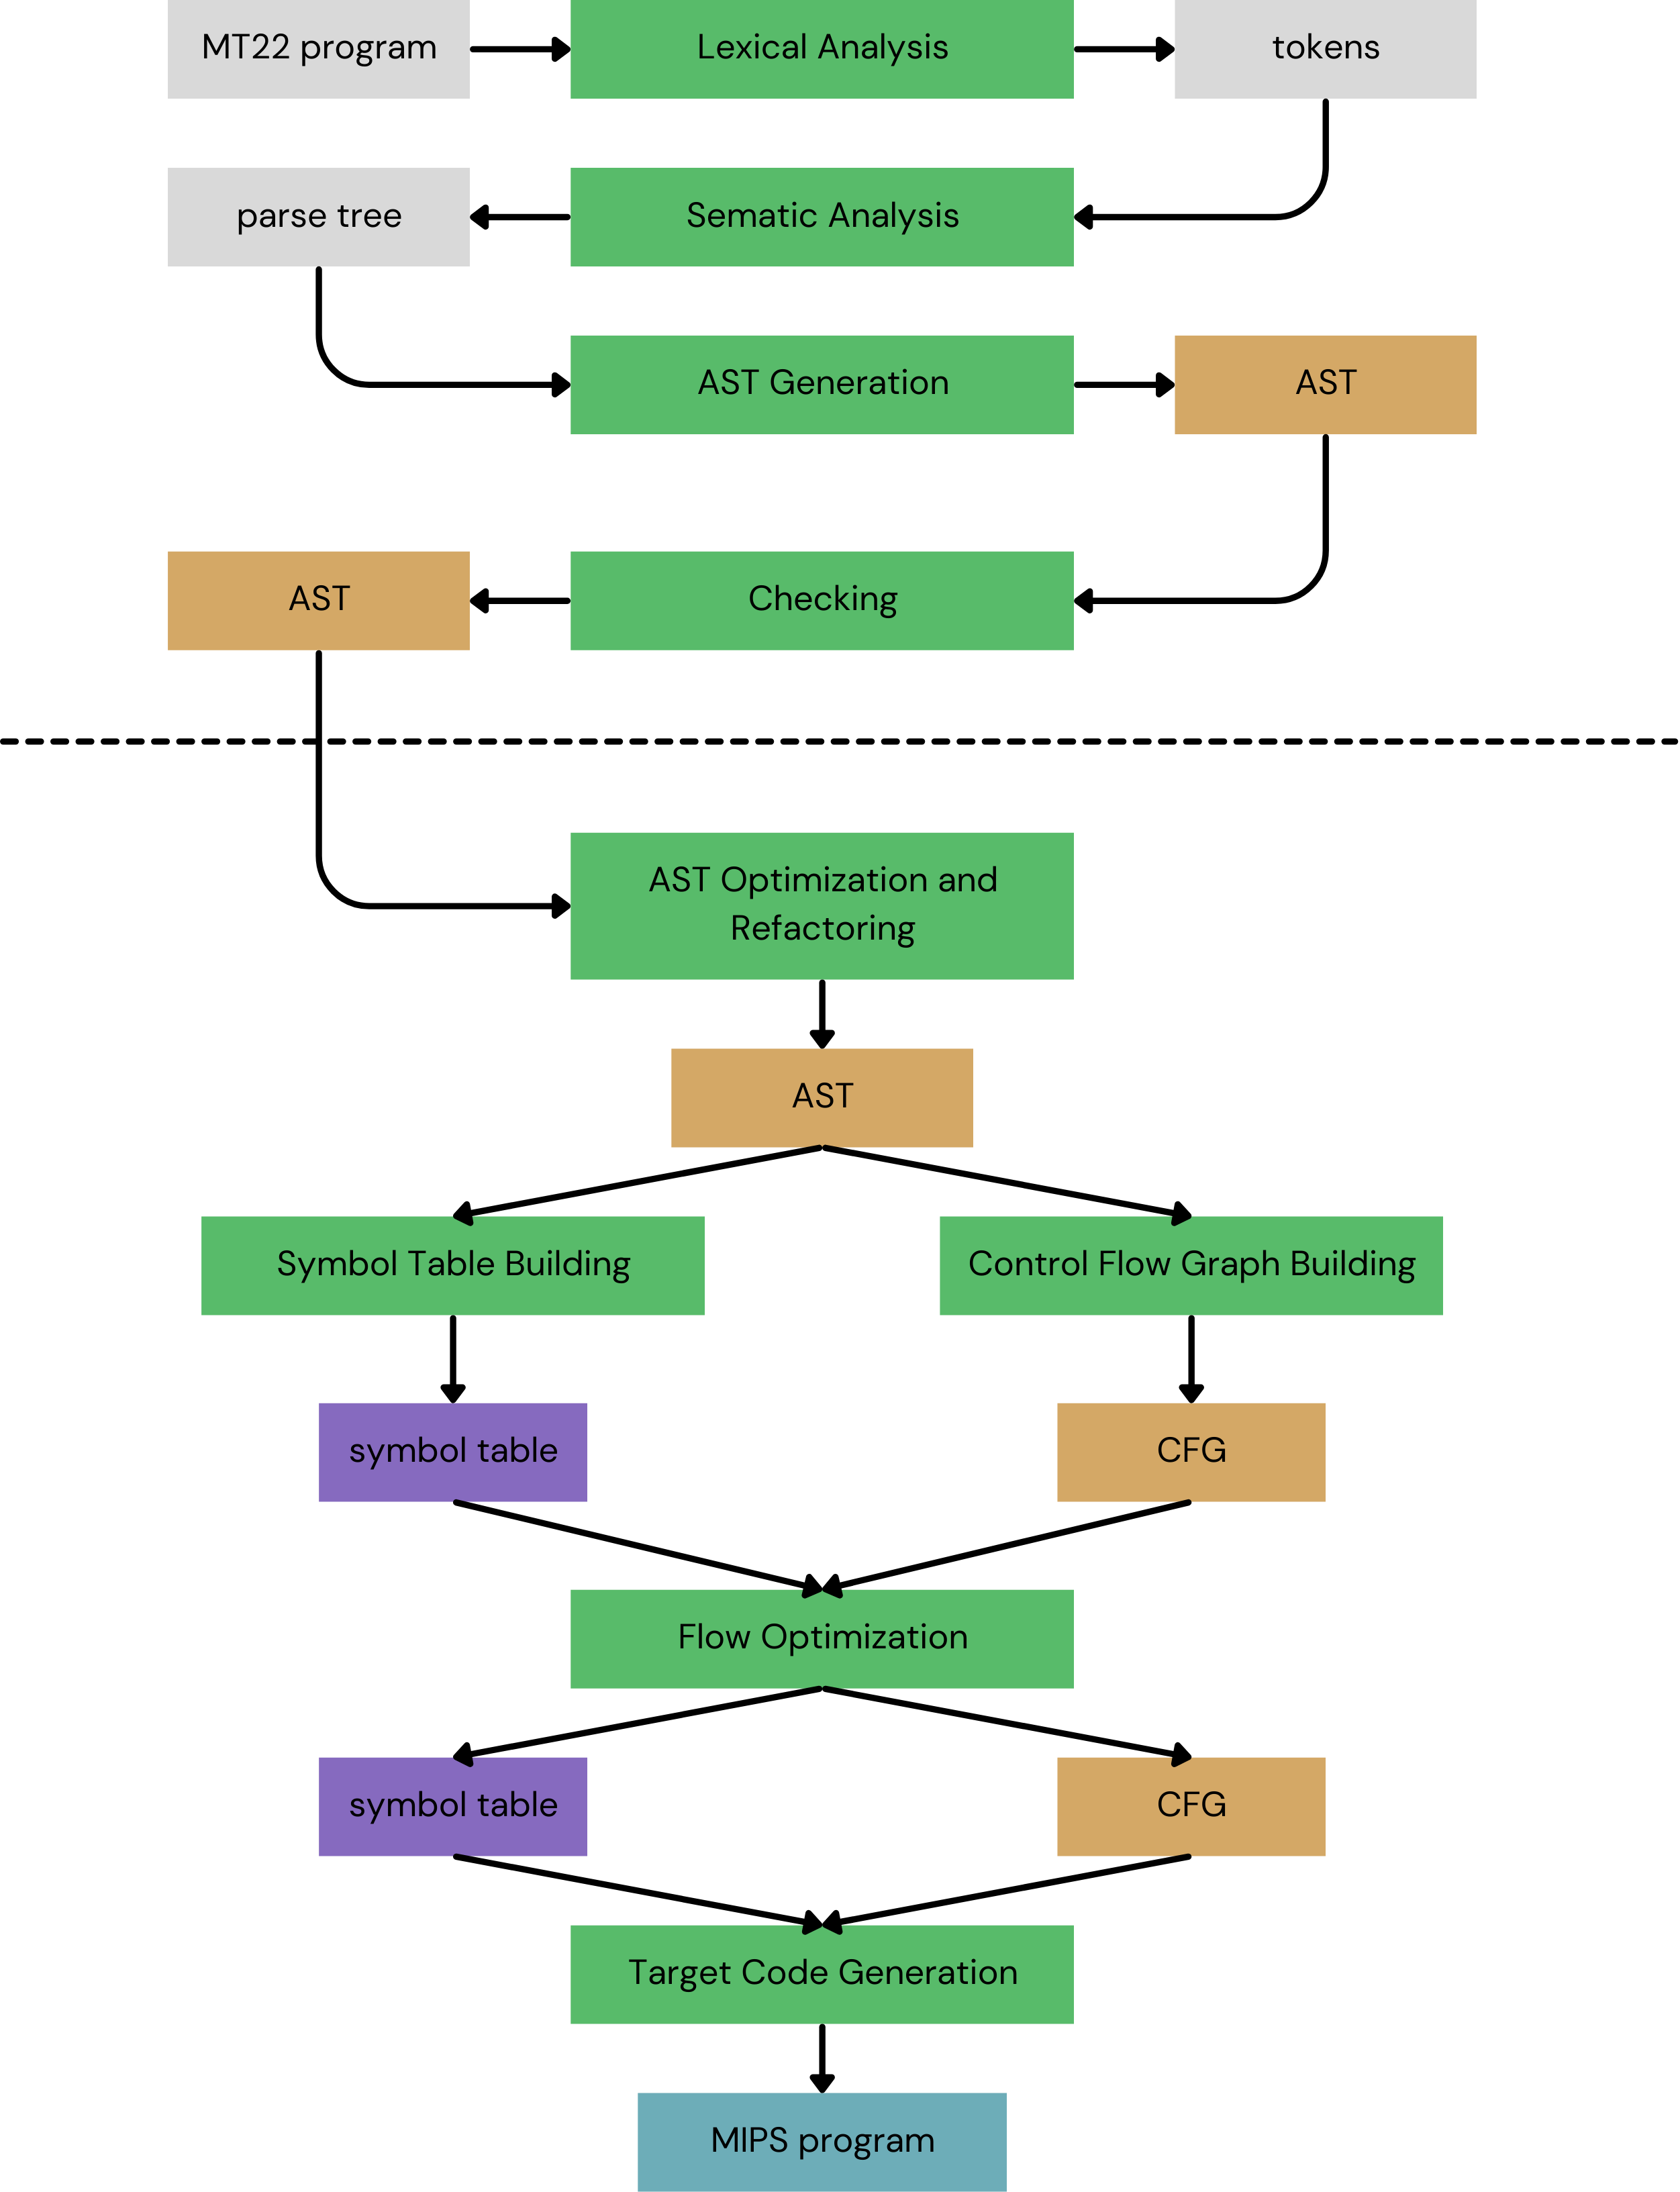
\includegraphics[width=0.8\textwidth]{img/compiler-phases.png}
    \caption{Phases of MT22-MIPS compiler}
    \label{figure:compiler-phases}
\end{figure}

Figure \ref{figure:compiler-phases} illustrates phases of the MT22-MIPS compiler, derived closely to general compilers. The dashed line separates between frontend and backend processes. The frontend has been implemented in class assignments. Here we focus on the backend. Abstract Syntax Tree (AST) is a well-known intermediate representation (IR) for our program, whose major nodes are shown in Figure \ref{figure:ast}. Note that BlockStmt, IfStmt, ForStmt, WhileStmt and DoWhileStmt include at least one Stmt. The AST is produced after the frontend process, then it is refactored and optimized one more time in the backend.

\begin{figure}[ht]
    \centering
    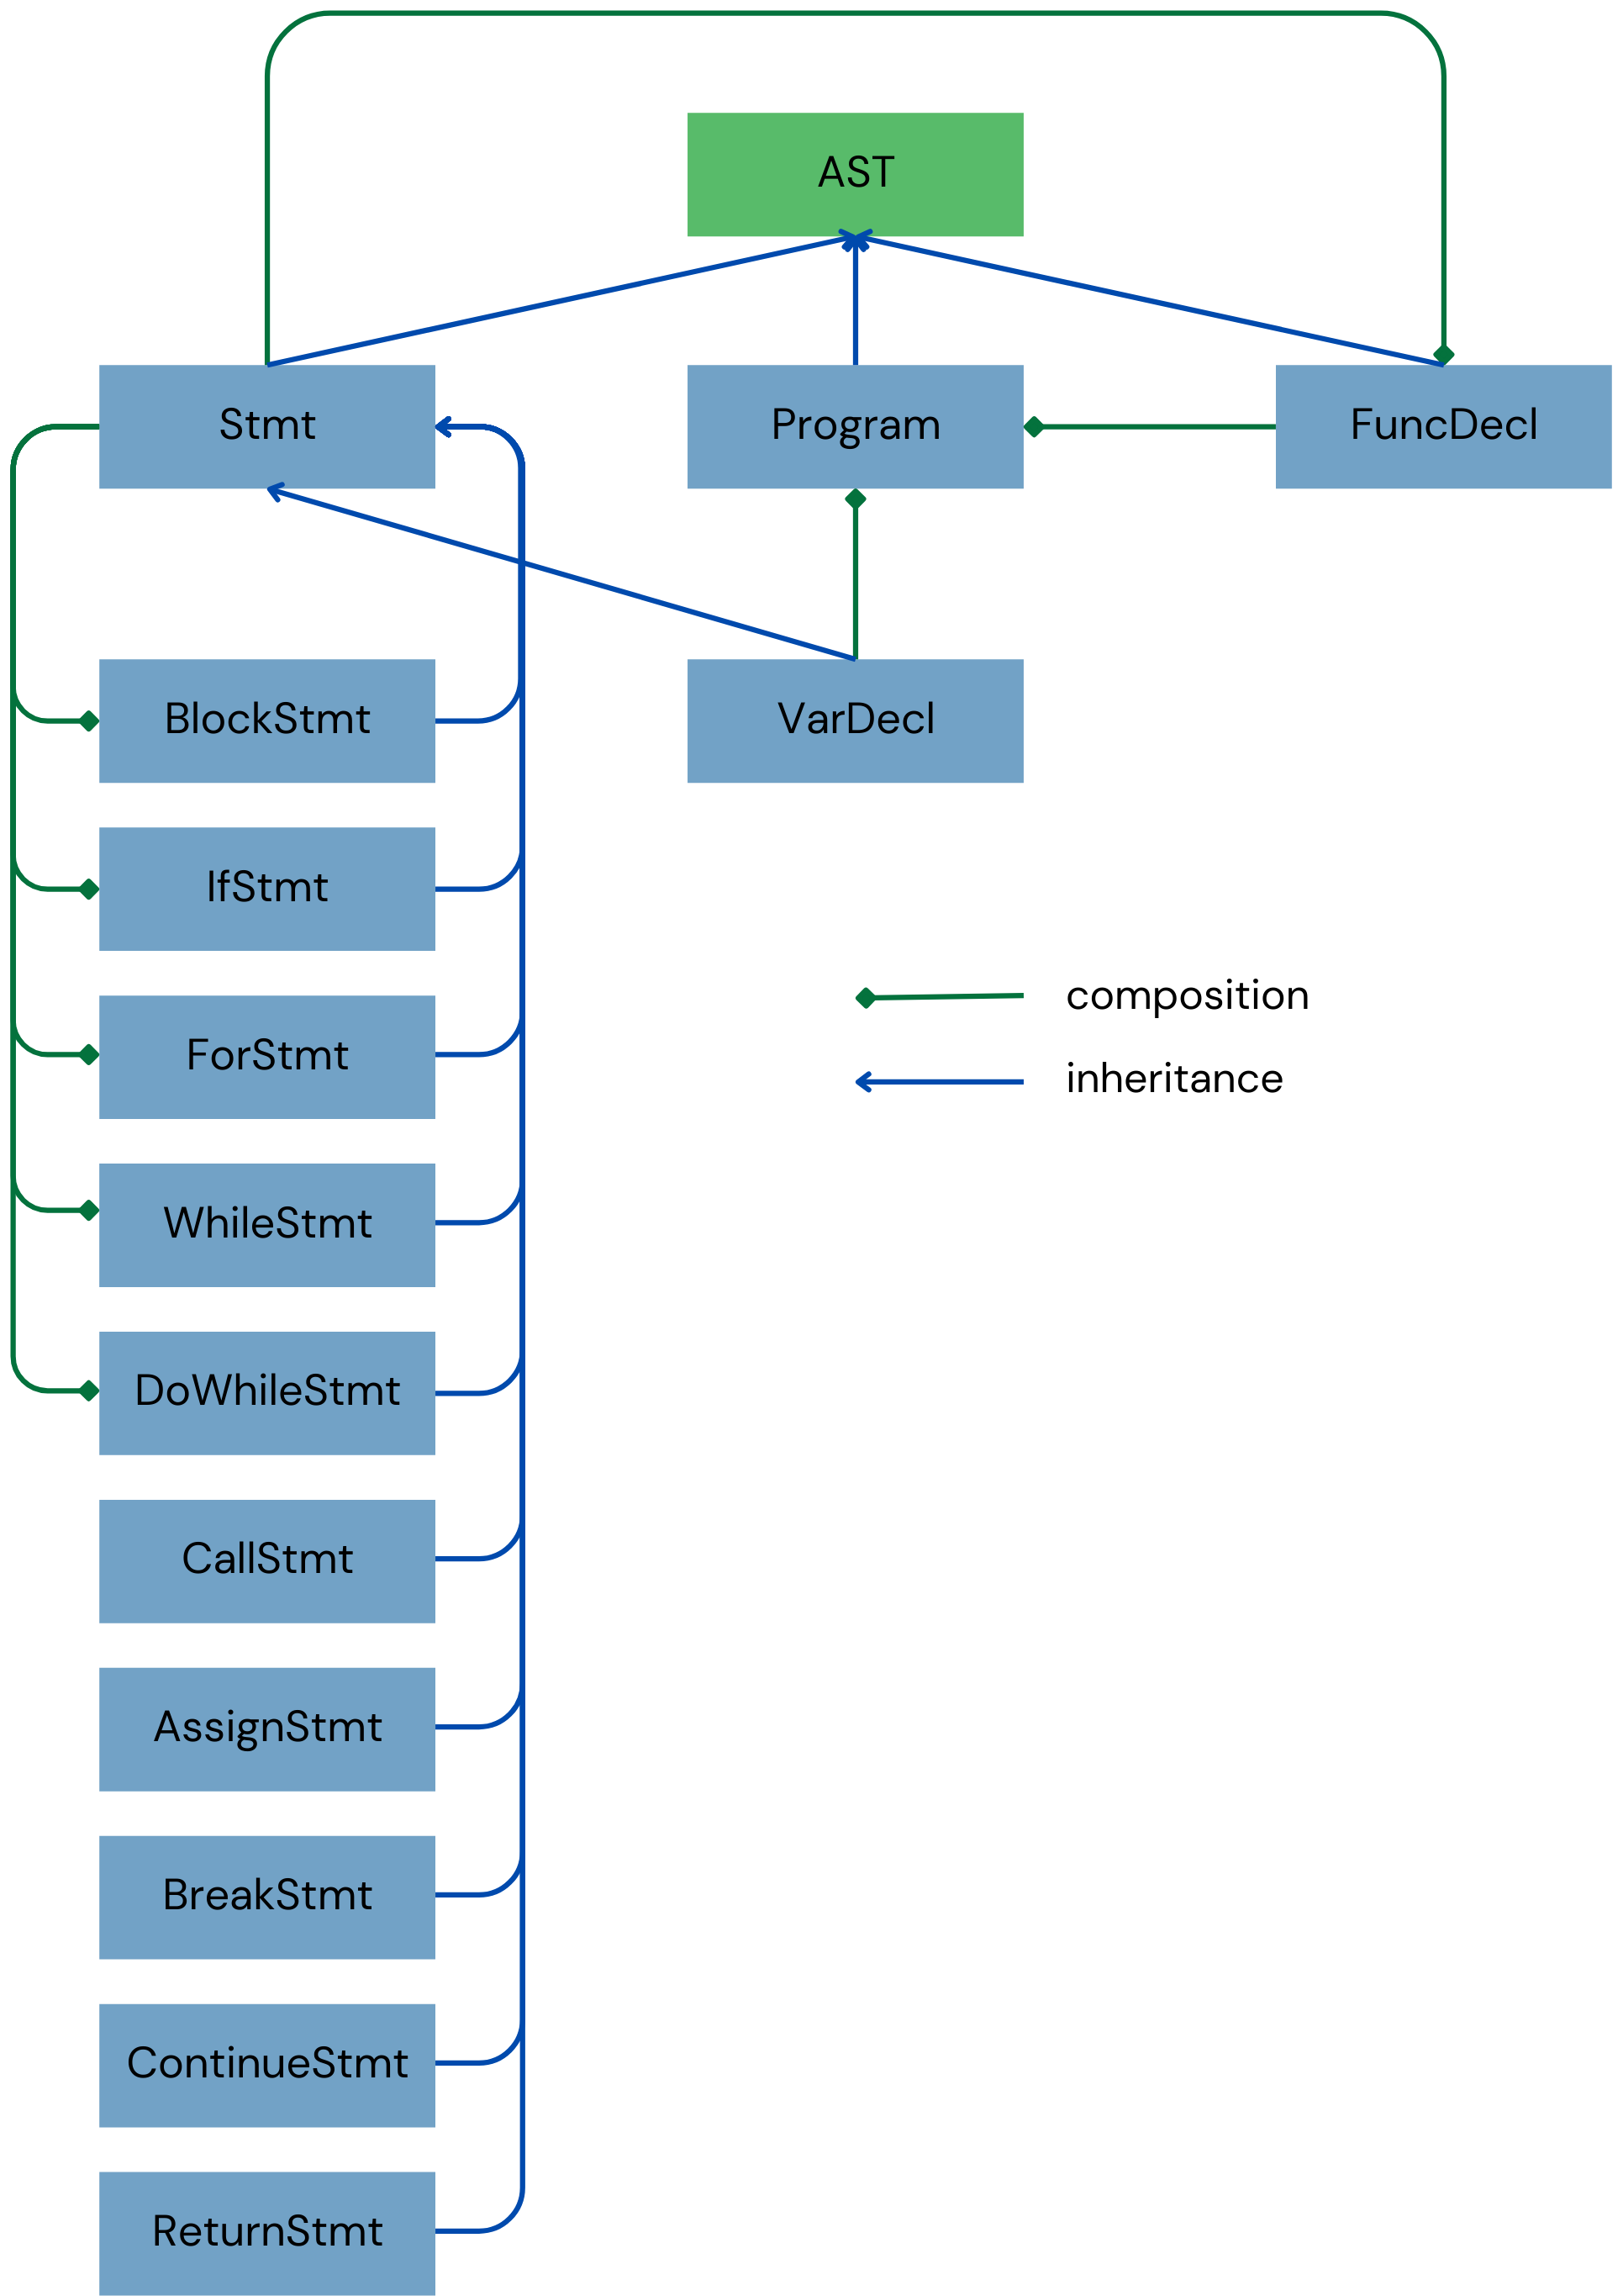
\includegraphics[width=0.7\textwidth]{img/ast.png}
    \caption{Overview of statement relations}
    \label{figure:ast}
\end{figure}

Another equivalent IR, the Control Flow Graph (CFG) and an assisting data structure, the Symbol Table. Flow Optimization and Target Code Generation work with the symbol table and the CFG.
\section{Backend Design}
We use the Visitor design pattern for phases and sub-phases in the backend, as shown in Listing \ref{listing:visitor-pattern}. Possible visitees are AST and CFG. Information is passed through visitors through a \texttt{VisitData} object. A visitor function takes the data from its caller and returns an \textit{updated data}. This strategy is to ensure purity and to let us visit a visitee just by visiting its children and do later work one-by-one. Python uses pass-by-reference mechanism for a user-defined class, so our implementation does not impact on memory usage. In practice, it is sufficient to encapsulate an object and a context in the data. For each visitor, we have to explicate the visit context. The backend design is illustrated in Figure \ref{figure:backend-design}

\begin{lstlisting}[language = python, caption={Visitor pattern}, label={listing:visitor-pattern}]
class VisitData:
    def __init__(self, 
                obj, # the object of data structure needed to be visited
                ctx, # context needed for a visit function to return the complete updated data
                ):
        # Initialization

class Visitee:
    def accept(self, visitor, visit_data):
        method_name = "visit{}".format(self.__class__.__name__)
        visit_function = getattr(visitor, method_name)
        return visit_function(self, data)

class ExampleVisitee(Visitee): pass

class Visitor:
    def visit(self, visitee, visit_data):
        return visitee.accept(self, data)
    
    def visitExampleVisitee(self, visitee, visit_data):
        '''
        Instructions...
        '''
        return updated_visit_data
\end{lstlisting}

\begin{figure}
    \centering
    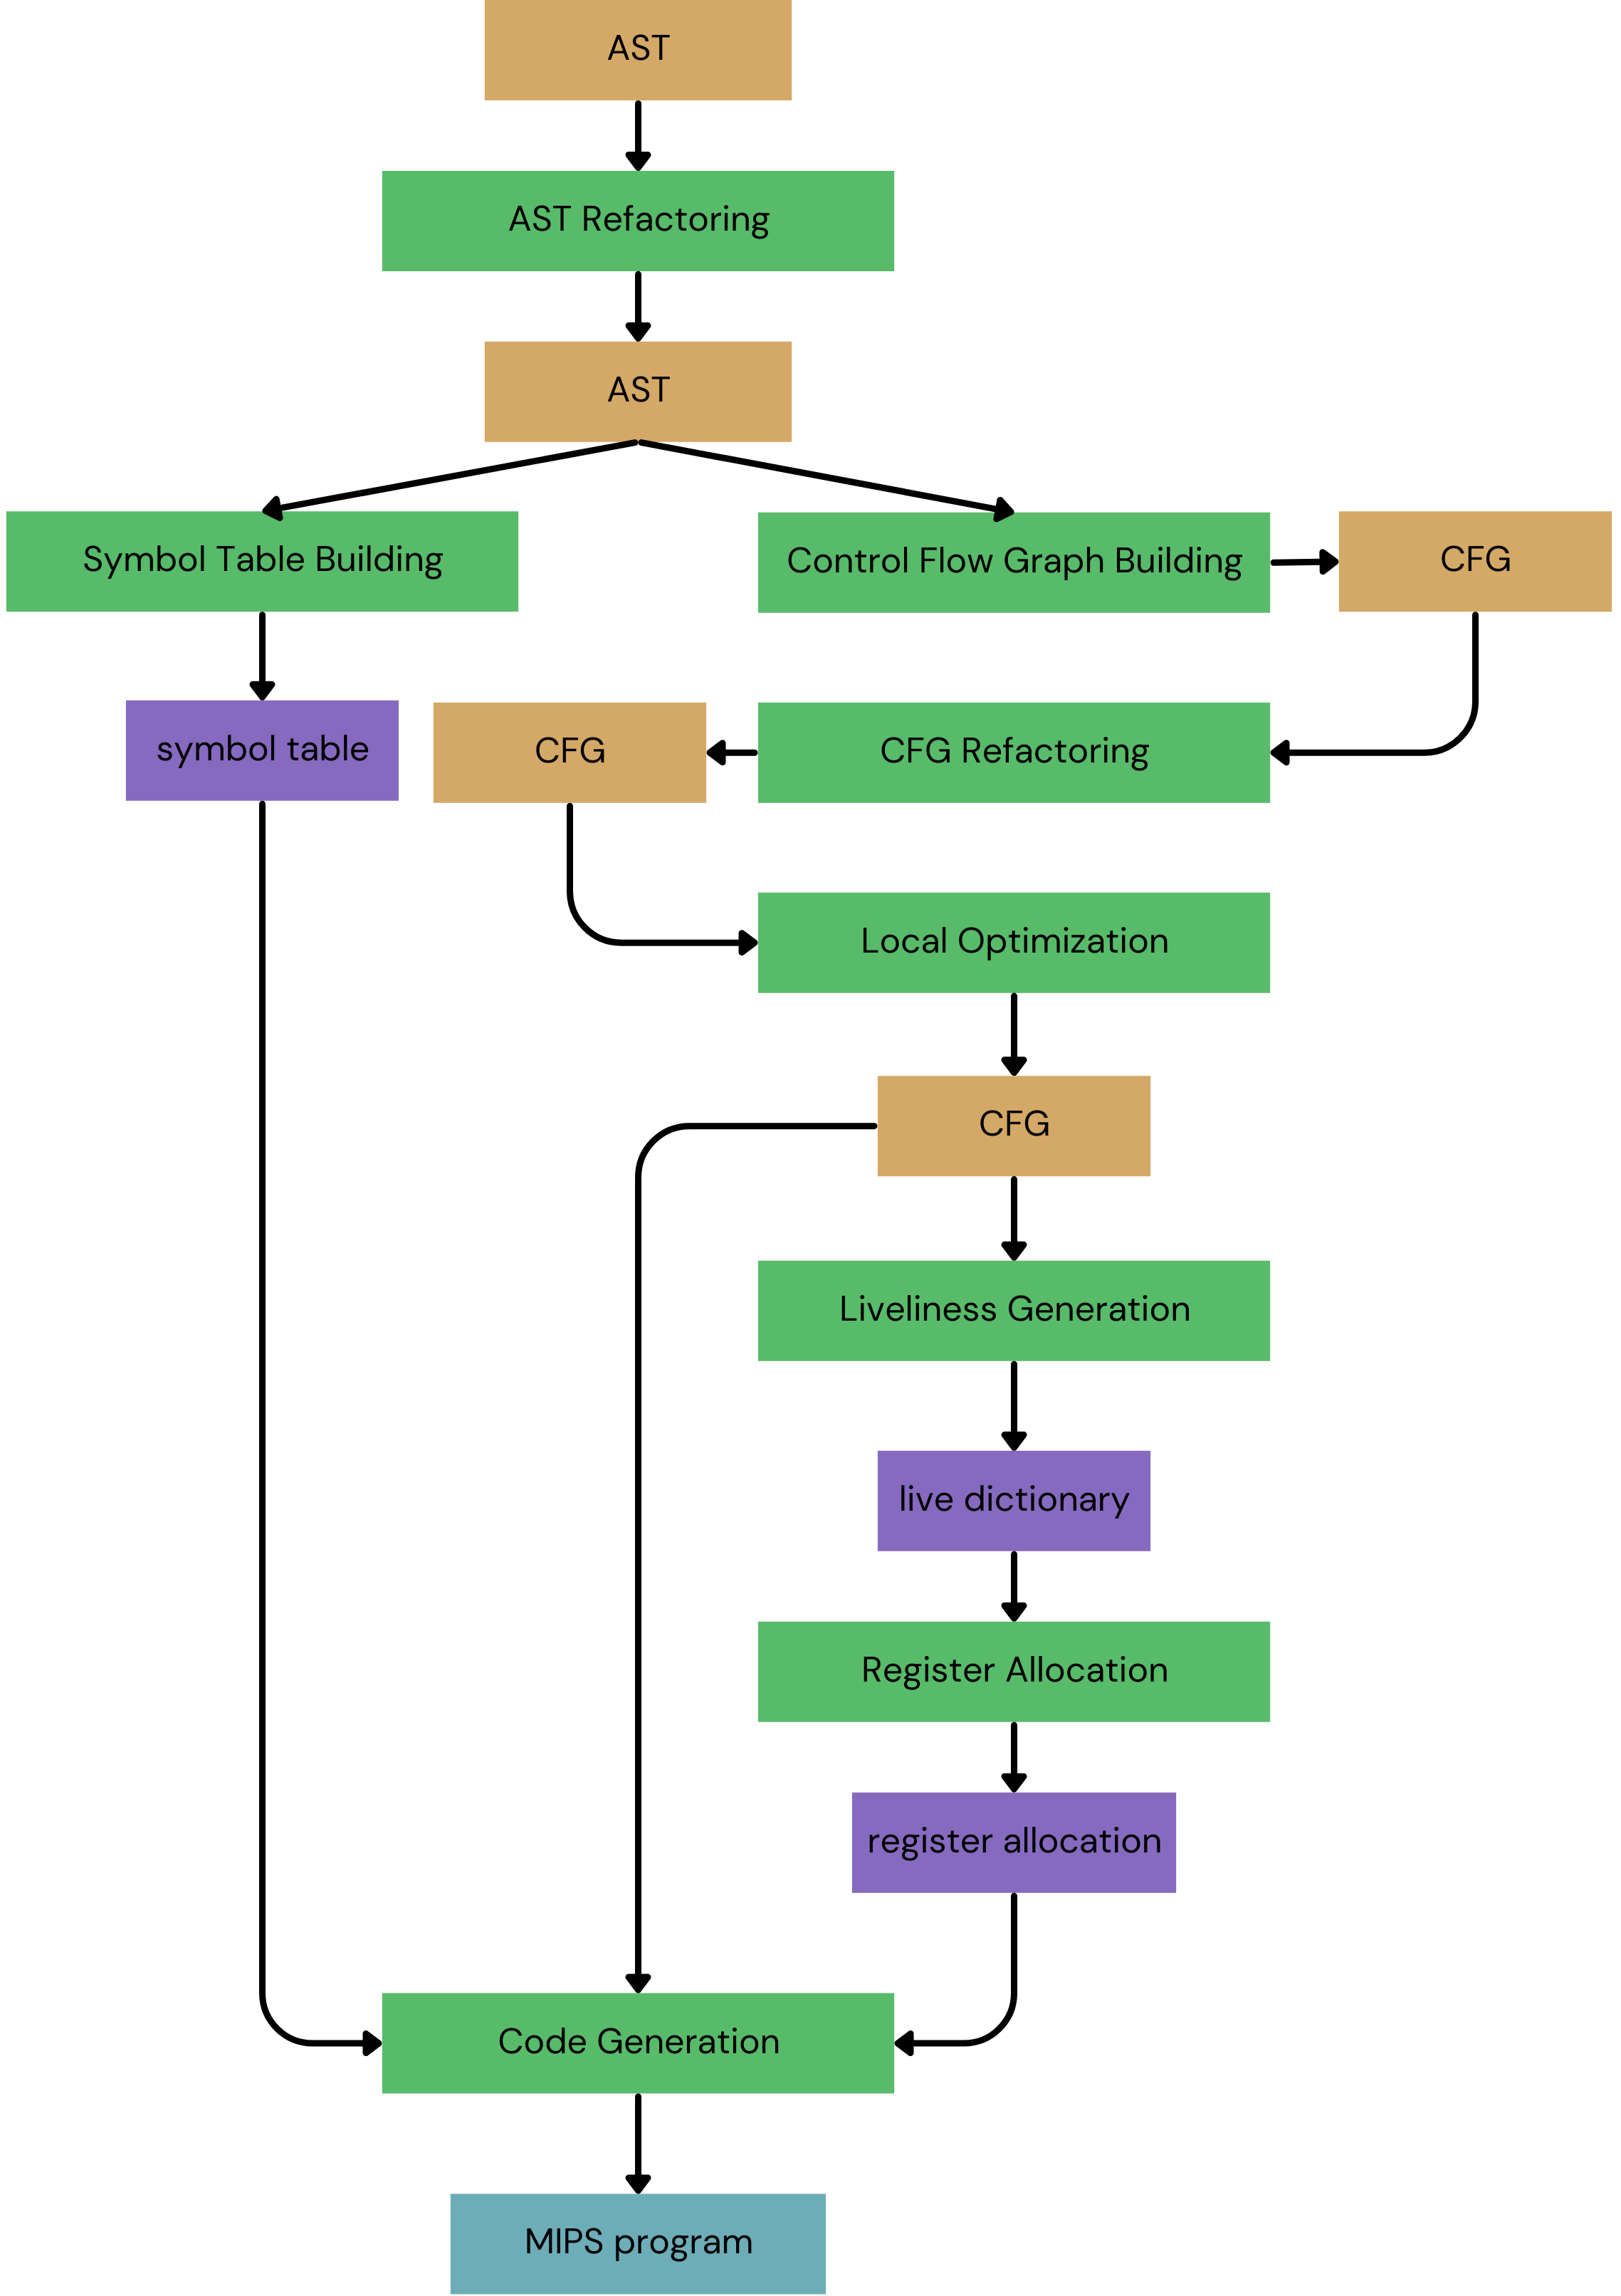
\includegraphics[width = 0.5\textwidth]{img/backend-design}
    \caption{Backend design}
    \label{figure:backend-design}
\end{figure}

\subsection{AST Refactor}

AST refactor modifies the AST in preparation for later processes. Since variable declaration before using has been checked in frontend, we only need statements that use these variables, while recorded their data types. To sum up, the Refactorer helps us:

\begin{itemize}
  \item Eliminate dead code after ReturnStmt in FuncDecl.
  \item Turn Stmt used in IfStmt, WhileStmt, ForStmt and DoWhileStmt to BlockStmt
  \item Remove VarDecl(name, type, value), while add the name into the symbol table.
  \item Turn VarDecl(name, type, value) to AssignStmt(Id(name), value, referenced\_type), while add the name into the symbol table.
  \item Turn ForStmt to WhileStmt.
  \item Unwrap complex BinExpr.
\end{itemize}

\begin{lstlisting}[language=Python]
class ASTRefactorContext:
class ASTRefactorerContext:
  def __init__(self, 
              last_sym # last symbol accessed by the last sub-expression, excluded to BinExpr unwrapper
              used_sum # the symbol that will be used by sub-expressions):
    # Initializations
\end{lstlisting}
\subsection{CFG Building}
A control flow graph (CFG) is composed of basic blocks. Each basic block contains a sequence of statements that can be executed sequentially. Listing \ref{listing:cfg} illustrates the design of CFG and the building context. High level implementations are shown in following figures.

\begin{lstlisting}[language = python, caption={CFG Design and its building context}, label={listing:cfg}]
  class Block(Visitee):
      def __init__(self, id, name,
                  stmts,  # list of statements in the block
                  cond,   # branching condition

                  next,   # next block on no condition

                  true,   # branched block on true condition
                  false,  # branched block on false condition

                  jump,   # jumped block on FuncCall or CallStmt
                  link,   # linked block after FuncCall or CallStmt
                  end,    # the block ending a FuncCall or CallStmt
                ):
          # Initialization
  
  class CFG(Visitee):
      def __init__(self, blocks, avail_id):
          # Initialization
          
          self.obj.blocks = [Block(id=0)]
  
          # context
          self.ctx.active_block = self.obj.blocks[-1] # any statements rather than IfStmt, WhileStmt and CallStmt will be added to this block when visited
  
          self.ctx.loop_block = None # , active_block points to this block if ContinueStmt is visited
  
          self.ctx.endloop_block = None # pointed to by a visited BreakStmt.

  class CFGBuilderContext:
      def __init__(self, 
                  active_block, # current active block
                  loop_block,   # the first block when entering a loop
                  endloop_block # the block after visit statements in loop
                  ):
          # Initialization
\end{lstlisting}

\begin{figure}
  \centering
  \begin{minipage}{0.45\textwidth}
    \begin{lstlisting}[language=python]
    # Last Block
    if (expr)
      tstmt
    else
      fstmt
    # Next Block
    \end{lstlisting}
  \end{minipage}%
  \hfill
  \begin{minipage}{0.45\textwidth}
    \centering
    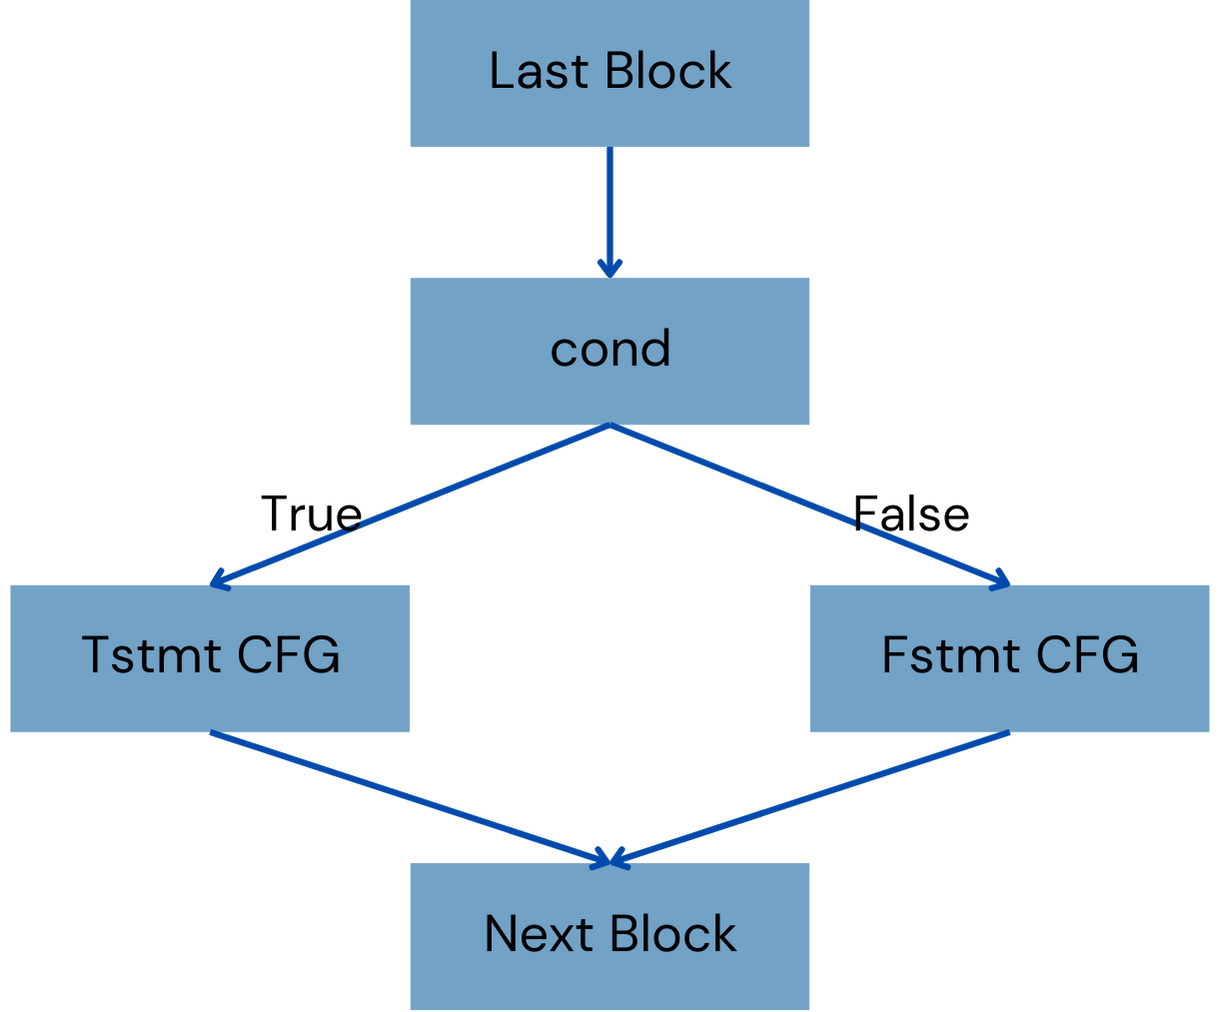
\includegraphics[width=0.9\textwidth]{img/ifstmt-cfg.png}
  \end{minipage}
  \caption{CFG of IfStmt}
\end{figure}

\begin{figure}
  \centering
  \begin{minipage}{0.45\textwidth}
    \begin{lstlisting}[language=python]
    # Last Block
    while (cond) {
      stmt
    }
    # Next Block
    \end{lstlisting}
  \end{minipage}%
  \hfill
  \begin{minipage}{0.45\textwidth}
    \centering
    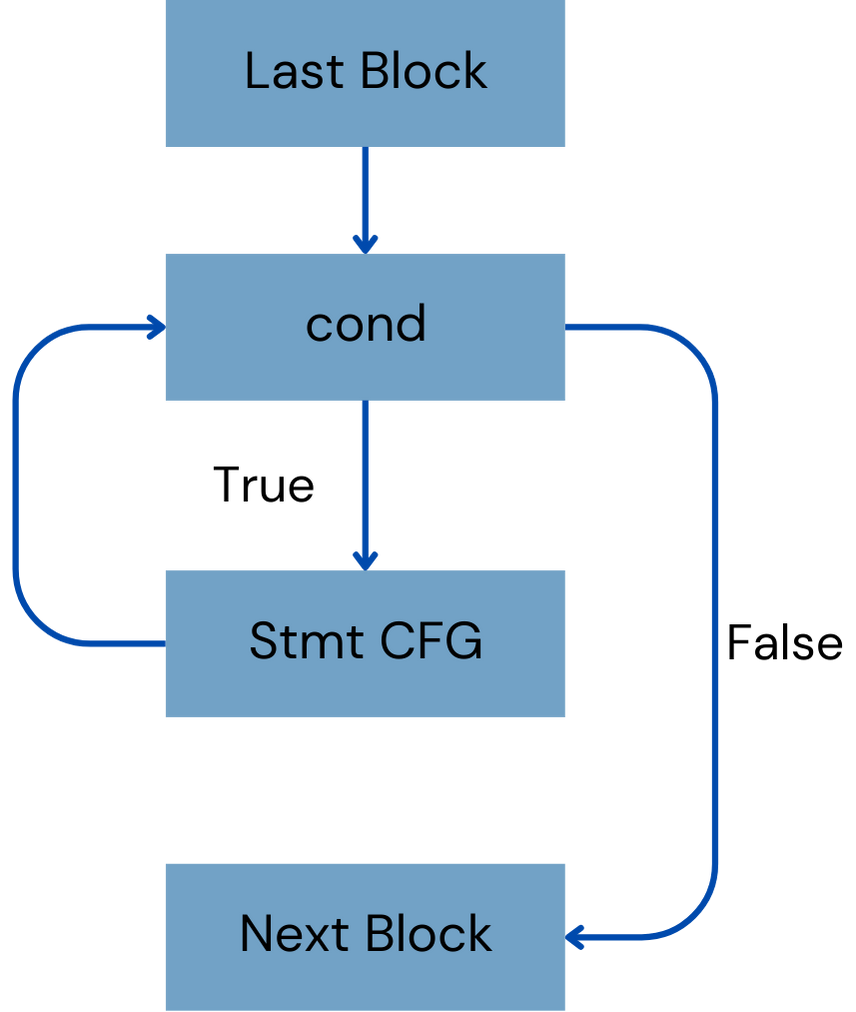
\includegraphics[width=0.9\textwidth]{img/whilestmt-cfg.png}
  \end{minipage}
  \caption{CFG of WhileStmt}
\end{figure}

\begin{figure}
  \centering
  \begin{minipage}{0.45\textwidth}
    \begin{lstlisting}[language=python]
    # Last Block
    do {
      stmt
    } while (cond)
    # Next Block
    \end{lstlisting}
  \end{minipage}%
  \hfill
  \begin{minipage}{0.45\textwidth}
    \centering
    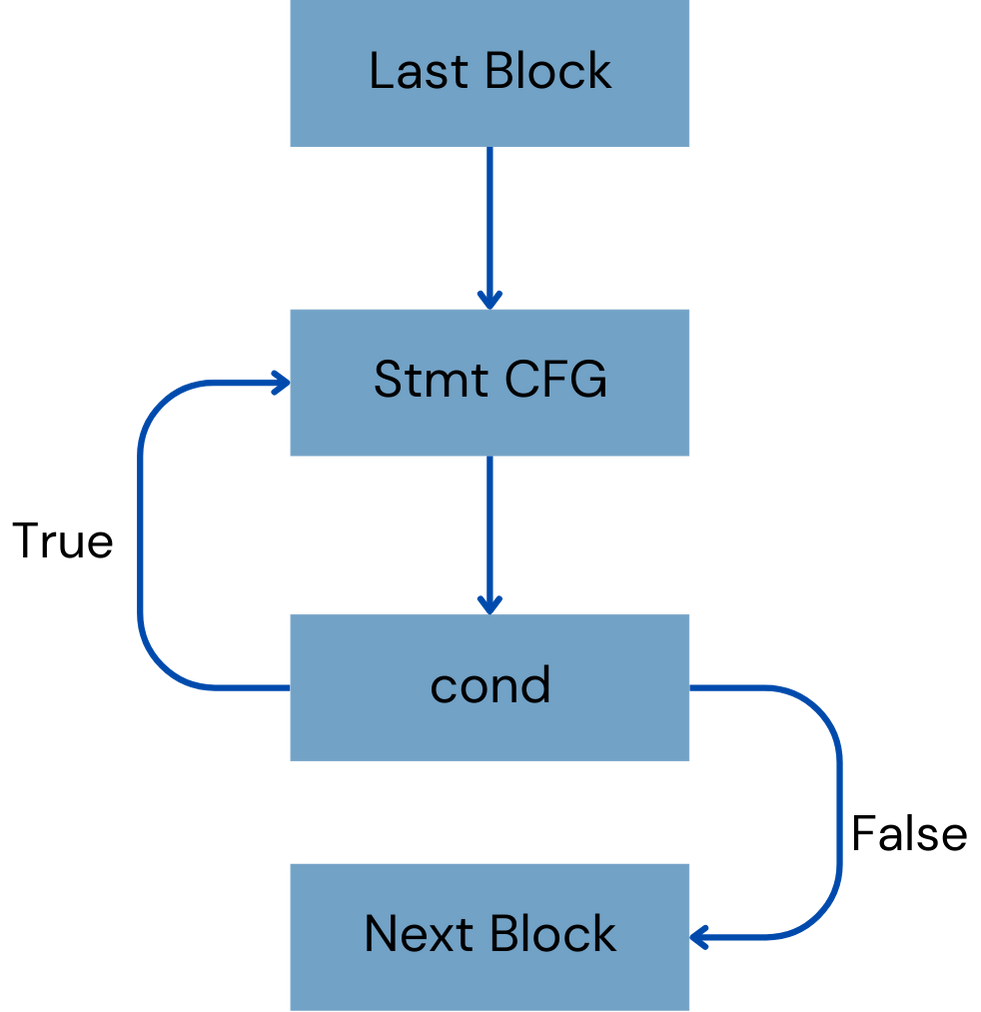
\includegraphics[width=0.9\textwidth]{img/dowhilestmt-cfg.png}
  \end{minipage}
  \caption{CFG of DoWhileStmt}
\end{figure}

% \begin{figure}
%   \centering
%   \begin{minipage}{0.45\textwidth}
%     \begin{lstlisting}[language=python]
%     # Last Block
%     for (assign, cond, update){
%       stmt
%     }
%     # Next Block
%     \end{lstlisting}
%   \end{minipage}%
%   \hfill
%   \begin{minipage}{0.225\textwidth}
%     \centering
%     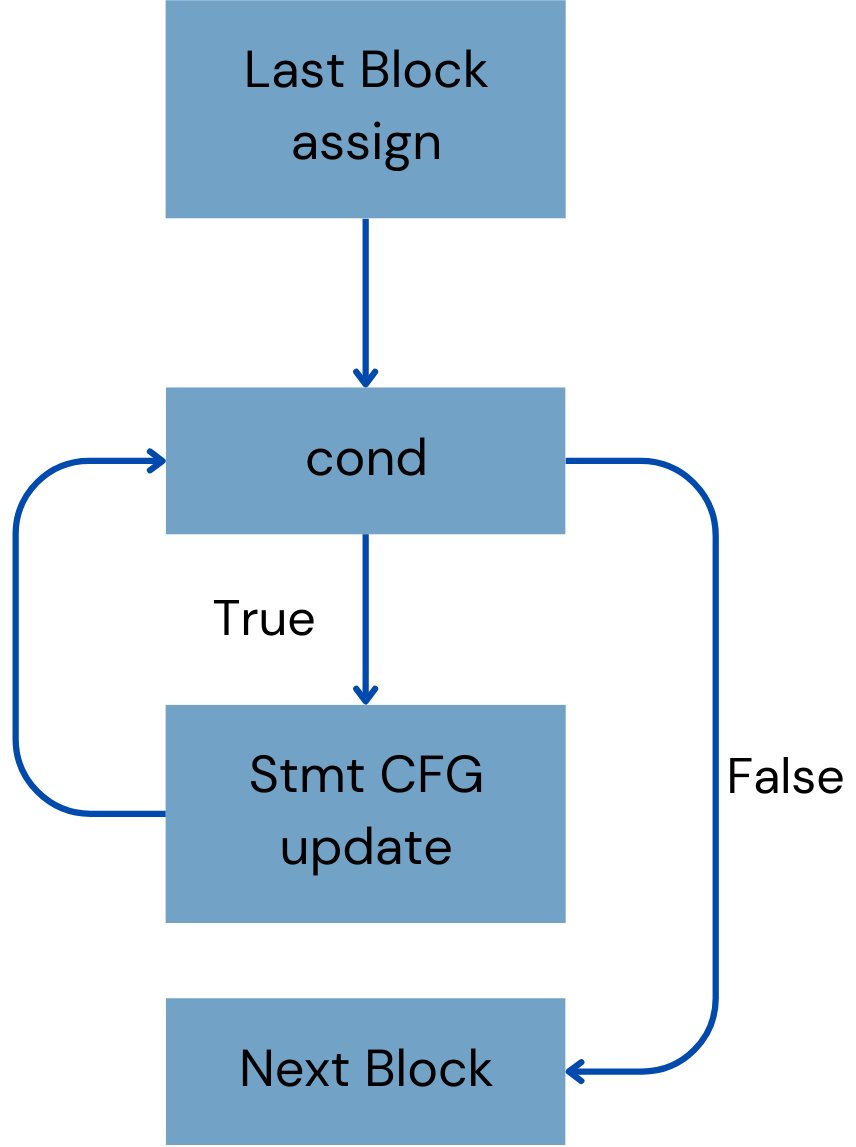
\includegraphics[width=0.9\textwidth]{img/forstmt-cfg.png}
%   \end{minipage}
%   \caption{CFG of ForStmt}
% \end{figure}

\begin{figure}
  \centering
  \begin{minipage}{0.45\textwidth}
    \begin{lstlisting}[language=python]
      func_name : function void ()
        body
      \end{lstlisting}
  \end{minipage}%
  \hfill
  \begin{minipage}{0.45\textwidth}
    \centering
    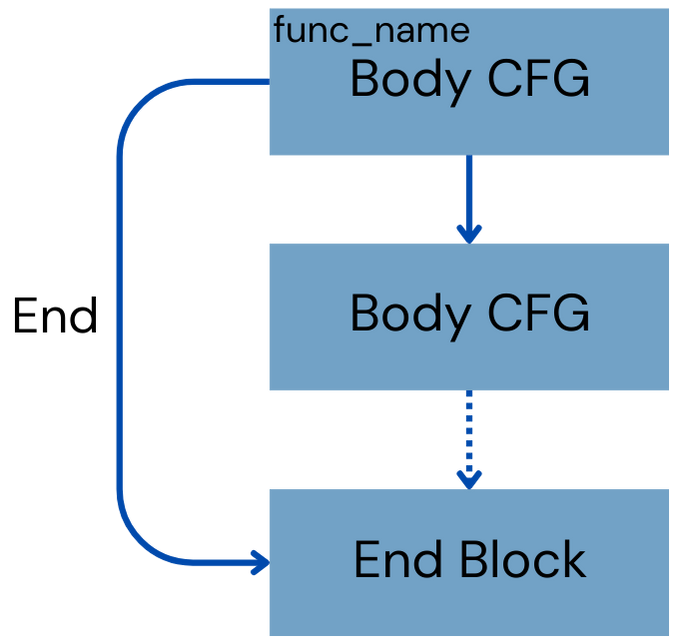
\includegraphics[width=0.5\textwidth]{img/funcdecl-cfg.png}
  \end{minipage}
  \caption{CFG of FuncDecl}
\end{figure}


\begin{figure}[ht]
  \centering
  \centering
  \begin{minipage}{0.45\textwidth}
    \begin{lstlisting}[language=python]
      # Last Block
      func_name(params)
      # Next Block
      \end{lstlisting}
  \end{minipage}%
  \hfill
  \begin{minipage}{0.45\textwidth}
    \centering
    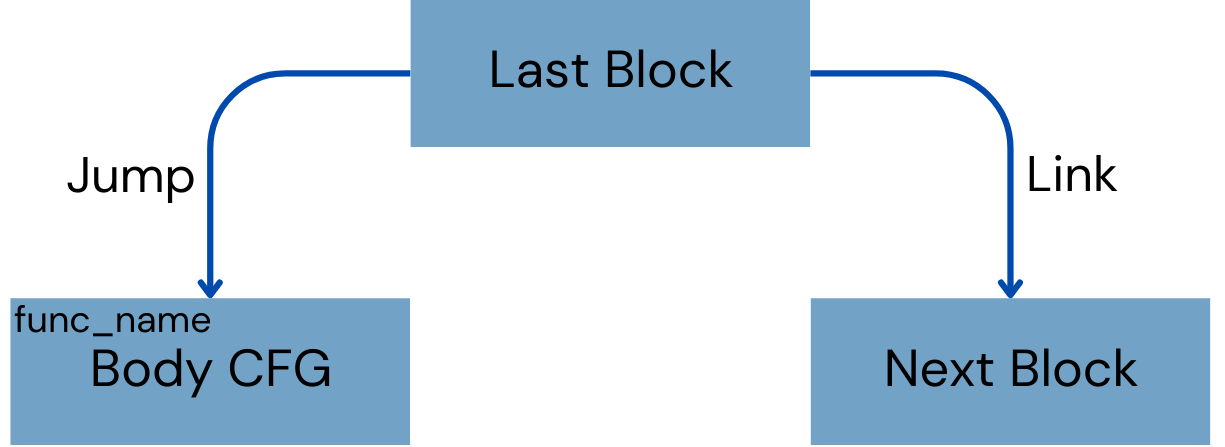
\includegraphics[width=0.9\textwidth]{img/call-cfg.png}
  \end{minipage}
  \caption{CFG of FuncCall and CallStmt}
\end{figure}

We see the structure of a CFG in Figure \ref{figure:cfg-structure}, much simpler than AST in statement types but dataflow expressible.

\begin{figure}[ht]
  \centering
  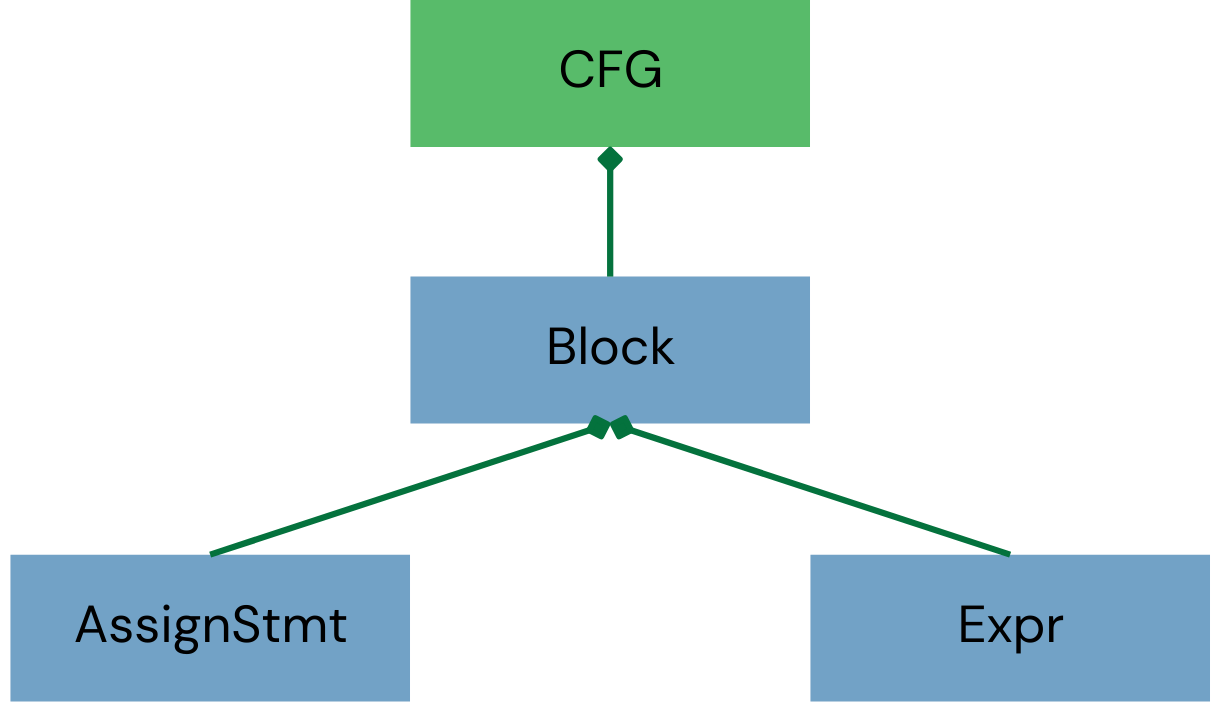
\includegraphics[width = 0.5 \textwidth]{img/cfg.png}
  \caption{The structure of a CFG}
  \label{figure:cfg-structure}
\end{figure}

\begin{figure}[ht]
  \centering
  \begin{minipage}[t]{0.4\textwidth} % Adjust the width here
    \begin{lstlisting}[language=Python]
data = '''
main : function void() {
a : array[5] of integer = {5,4,3,2,1};
tmp : integer;
for (i = 0; i < 4; i = i + 1){
  for (j = i+1; j < 5; j = j + 1) {
    if (a[i] > a[j]) {
      tmp = a[i];
      a[i] = a[j];
      a[j] = tmp;
    }
  }
}
}
'''
\end{lstlisting}
  \end{minipage}
  \hfill
  \begin{minipage}[t]{0.55\textwidth}
    \begin{lstlisting}[language=Python]
'''
Program([
  Func(main, void, [], None, 
    Block([
      Assign(a, [5, 4, 3, 2, 1]),
      Assign(i, 0.0),
      While(BinExpr(<, i, 4), 
        Block([
          Assign(j, BinExpr(+, i, 1)),
          While(BinExpr(<, j, 5), 
            Block([
              If(BinExpr(>, ArrayCell(a, [i]), ArrayCell(a, [j])), 
              Assign(tmp, ArrayCell(a, [i]))),
              Assign(ArrayCell(a, [i]), ArrayCell(a, [j])),
              Assign(ArrayCell(a, [j]), tmp),
              Assign(j, BinExpr(+, j, 1))
            ])),
          Assign(i, BinExpr(+, i, 1))]))]))
])
'''
\end{lstlisting}
  \end{minipage}
  \vfill
  \begin{minipage}[t]{\textwidth}
    \centering
    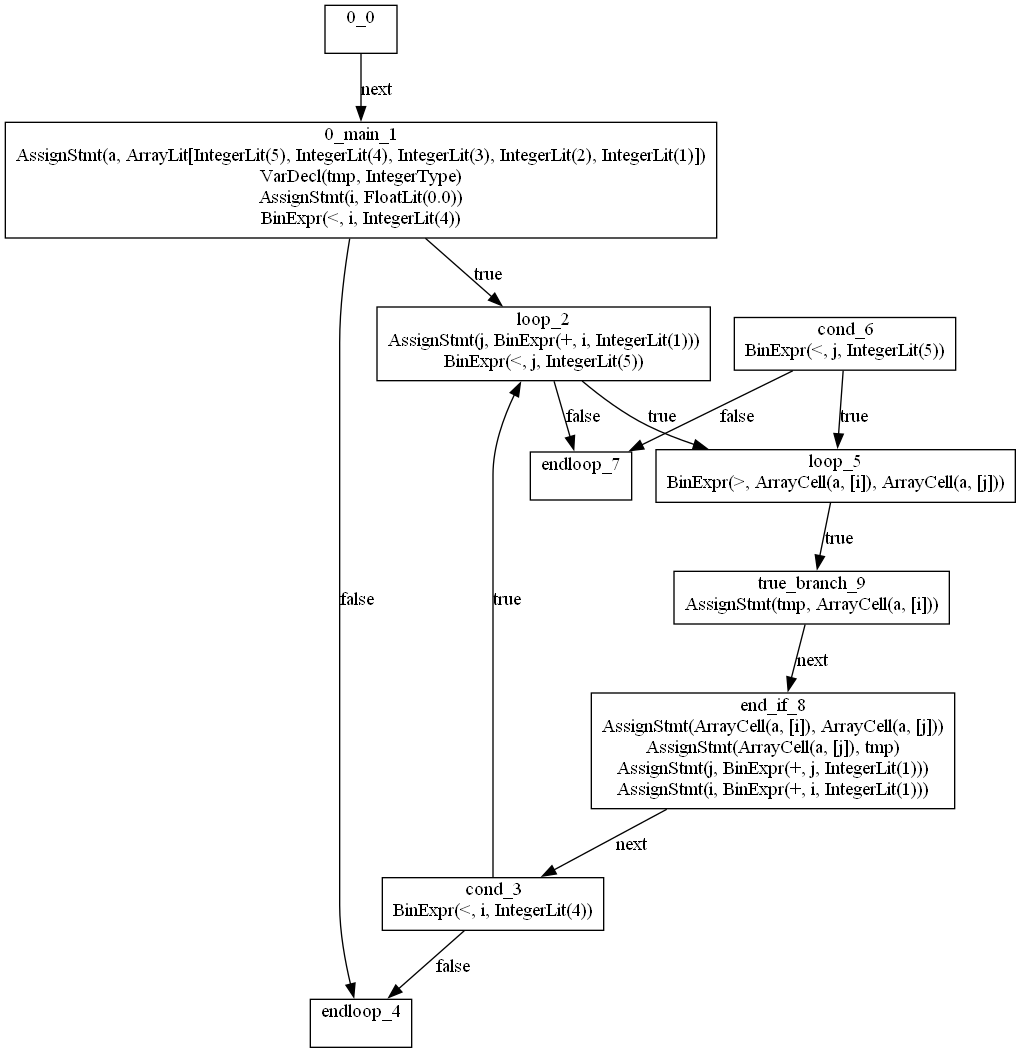
\includegraphics[width=0.8\textwidth]{img/cfg-example.png}
  \end{minipage}
  \caption{A MT22 program, its refactored AST and its corresponding CFG (rendered with Graphiz)}
\end{figure}

\subsection{CFG Refactor}
This component simply remove empty block out of the CFG.
\subsection{CFG Local Optimization}
Local Optimizer includes
\begin{itemize}
  \item Algebraic Simplification: whenever there is \texttt{Expr} of all literals, compute beforehand if possible.
  \item Copy Propagation: whenever there is \texttt{AssignStmt(Id(x), Id(y))}, replace all future usages of \texttt{x} by \texttt{y} until the next assignment of \texttt{x}.
  \item Constant Folding: whenever there is \texttt{AssignStmt(Id(x), literal)}, replace all future usages of \texttt{x} by \texttt{y} until the next assignment of \texttt{x}.
  \item Dead Code Elimination: \texttt{AssignStmt(Id(x), Id(y))} and \texttt{x} does not appear elsewhere in the block, delete this statement.
\end{itemize}

Each component is implemented as a CFG Visitor, which returns an updated CFG. The components are run iteratively until no changes appear.

\subsection{Liveliness Generation}
Liveliness is a determination of usage of the symbols. A symbol $x$ is live at statement $s$ if
\begin{enumerate}
  \item There exists a statement $s'$ that uses $s$.
  \item There is a path from $s$ to $s'$ in the CFG.
  \item From $s$ to $s'$, there is no re-assignment of $x$.
\end{enumerate}
We compute liveliness by passing live information through adjacent statements through a function
$$L(s,x, \text{in | out}).$$
This function determines whether a symbol $x$ is live incoming or outcoming of a statement $s$. We follow these rules:
\begin{enumerate}
  \item If a condition $C$ uses $x$, then $x$ is live incoming this assignment.
        \begin{equation}
          L(C(x), x, \mathrm{in}) = \mathrm{True}.
        \end{equation}
  \item If an assignment uses $x$ on the right-hand side, then $x$ is live incoming this assignment.
        \begin{equation}
          L(\ldots := \mathrm{LHS}(x), x, \mathrm{in}) = \mathrm{True}.
        \end{equation}
  \item If an assignment refers to $x$ on the left-hand side but not the right-hand side, then $x$ is not live incoming this assignment
        \begin{equation}
          L(x := e, x, \mathrm{in}) = \mathrm{False}.
        \end{equation}
  \item If a statement does not refer to $x$, then the liveliness of $x$ does not change when outcoming the statement.
        \begin{equation}
          L(s, x, \mathrm{in}) = L(s, x, \mathrm{out})
        \end{equation}
  \item If $x$ is live incoming a statement $s'$, then $x$ is live outcoming predecessors of $s'$.
        \begin{equation}
          L(s, x, \mathrm{out}) = \bigvee \left\{ L(s',x,\mathrm{in}) : s' \text{ is a successor of }  s\right\}.
        \end{equation}
\end{enumerate}

The first three rules are run once. After that, the last two rules are run iteratively until no changes appear on the liveliness dictionary. After that, live symbols at each statement \texttt{stmt} is computed as all live symbols outcoming of this statement and incoming of its successor. In implementation, we remove all \texttt{VarDecl} as the declaration of a symbol when it is used has been checked.

\begin{lstlisting}[language = python, caption={Liveliness generator context}, label={listing:live-gen-context}]
  class LiveGenContext:
    def __init__(self, 
                  stmt,            # current visited statement
                  refered_symbols  # current refered symbols
                ):
    # Initialization
\end{lstlisting}

\subsection{Register Allocation}
Up to now, we have live symbols at every statement. Two symbols cannot be allocated to the same register if they are live at the same time. Hence, we construct a Register Inference Graph (RIG). Each symbol is represented by a node. There is an edge between two nodes if they are live simultaneously at some point in the program. Since register allocation is NP hard, we follow a heuristic approach. Generally, we try to allocate register to node whose degree is less than or equal to the number of register, then remove this node from RIG, and so on. If such node is not found, we spill the highest-degree node i.e. load and store continuously for respective symbol.

\begin{algorithm}
  \caption{Heuristic Register Allocation}
  \begin{algorithmic}
    \STATE $r$ : number of registers
    \STATE $G$ : register inference graph
    \STATE $S$ : empty stack

    \WHILE{$\text{rig.nodes is not empty}$}
    \STATE lst := nodes of degree less than or equal to $r$
    \IF{lst is empty}
    \STATE Spill the highest-degree node $N$
    \STATE Remove $N$ from $G$
    \ELSE
    \STATE Add highest-degree node $N$ in lst to $S$
    \STATE Remove $N$ from $G$
    \ENDIF
    \ENDWHILE

    \WHILE{$S$ is not empty}
    \STATE choose appropriate register for $N$
    \ENDWHILE
  \end{algorithmic}
\end{algorithm}
\subsection{Code Generation}
Until this point, we got registers allocated to our symbols. The binary expressions are also unwrapped. The Code Generator simply adds all unallocated symbols to memory and uses respective registers for allocated ones.




\section{Testing}
Command line testing with manual match has been provided in README file in the project \href{https://github.com/mintcd/compiler-design.git}{repository}.

\printbibliography
\end{document}